\documentclass[../main]{subfiles}

\begin{document}

\subsection{Generative Adversarial Networks}

\subsubsection{Basic GAN Architecture}

The first GAN architecture was proposed in 2014, in the paper "Generative Adversarial Nets" by Goodfellow, et al.  Its architecture fulfills the basic principle of the min-max game, as described above. Two neural networks, the Generator, and the Discriminator work against one another: the Generator aims to generate samples resembling real-world samples closely enough to fool the Discriminator, who tries to distinguish between the fake, generated samples and the real-world data. The underlying principle of this architecture is that the Generator approximates a transformation function, which maps a random input distribution to the distribution underlying real data samples. On the other hand, the Discriminator approximates the distance between the generated sample and the real underlying distribution.  \cite{goodfellow2014generative} \cite{Wang2019}

For a GAN to converge, it is necessary to reach Nash equilibrium between the Generator and Discriminator. In game theory, the Nash equilibrium describes the state where both players' strategies are optimal, considering the other player's strategy.  However, GANs are typically optimized using Stochastic Gradient Descent. As SGD isn't designed to find this equilibrium between Generator and Discriminator, basic GANs can suffer from failure to converge \cite{goodfellow2018}. If the Discriminator outperforms the Generator by too much,  vanishing gradients may occur,  impeding convergence. If the roles are reversed and the Generator consistently fools the Discriminator, training may continue after the point of optimality, worsening results. Another common issue with GANs is mode collapse, which occurs when the Generator generates a successful example and cannot deviate from this, thus only generating the same example repeatedly.

\subsubsection{Wasserstein GANs \cite{wgans}}
There are various changes to the standard GAN architecture that address its problems with slow convergence, lack thereof, and mode collapse. A widely accepted improvement is the use of Wasserstein Distance (\enquote{\textit{Earth Mover's Distance}}), instead of the Jensen-Shannon Divergence used in a vanilla GAN, as a loss function.  In a standard GAN, the JS Divergence measures the distance between the real sample distribution and that of the fake samples generated by the Generator. During Discriminator training, this distance should then be minimized. In WGANs the Discriminator is transformed to what the authors call \textit{The Critic}. Instead of discriminating between real and fake samples, the Critic merely scores its input sample on how real it is.  

The advantage of WGANs lies in the continuously differentiable Earth Mover's Distance, which allows for the Critic to be trained to optimality without risking vanishing gradients, as is the case in the vanilla architecture.  As the antagonist to the Generator is defined differently, there is no need to reach Nash equilibrium, thus stabilizing training. The issue of mode collapse is alleviated, as well. 
 
\subsubsection{Conditional GANs \cite{cgans}}
After GANs proved to be an effective tool for artificial image generation, the desire to directly modify the image class arose. Conditional GANs allow for this modification by training both Discriminator and Generator on an additional input parameter.  This parameter is simply concatenated with the input sample to either component while training occurs as usual.

\begin{figure}[h]
	\centering
	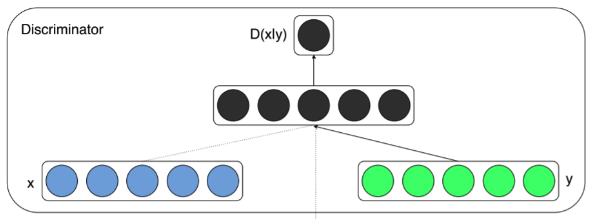
\includegraphics[scale=0.32]{cgan_1}
	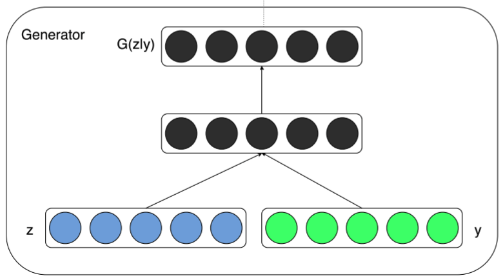
\includegraphics[scale=0.32]{cgan_2}
	\caption{The Conditional GAN Generator and Discriminator Components.  Where $x$ denotes the training sample, $y$ is the additional parameter,  	and $z$ is a random noise input}
\end{figure}


\subsection{Variational Autoencoders}
The Variational Autoencoder is an adaptation of the basic Autoencoder, allowing for more advanced sample generation.  The architecture of autoencoders consists of an encoder component and a decoder component, both neural networks. The goal of the autoencoder during training is for its output to correspond to its input,  while not simply learning the identity function. To achieve this, the data is passed through the encoder to a bottleneck, the embedding layer, only for this to be transformed to the original input by the decoder. At the embedding layer, the input data is now compressed while still capturing the essential characteristics of the input. 

Variational Autoencoders build upon this architecture by additionally learning the underlying distribution of the embeddings. Using the reparameterization trick, i.e. assuming an underlying Gaussian distribution,  noisy samples can now be generated from the embedding, allowing for variations on the original inputs. \cite{vaes}



\end{document}